
%%%%%%%%%%%%%%%%%%%%%%%%%%%%%%%%%%%%%%%%%%%%%%%%%%%%%%%%%%%%%%%%%%%%%
%% This is a (brief) model paper using the achemso class
%% The document class accepts keyval options, which should include
%% the target journal and optionally the manuscript type.
%%%%%%%%%%%%%%%%%%%%%%%%%%%%%%%%%%%%%%%%%%%%%%%%%%%%%%%%%%%%%%%%%%%%%
\documentclass[journal=jpccck,manuscript=suppinfo]{achemso}

%%%%%%%%%%%%%%%%%%%%%%%%%%%%%%%%%%%%%%%%%%%%%%%%%%%%%%%%%%%%%%%%%%%%%
%% Place any additional packages needed here.  Only include packages
%% which are essential, to avoid problems later. Do NOT use any
%% packages which require e-TeX (for example etoolbox): the e-TeX
%% extensions are not currently available on the ACS conversion
%% servers.
%%%%%%%%%%%%%%%%%%%%%%%%%%%%%%%%%%%%%%%%%%%%%%%%%%%%%%%%%%%%%%%%%%%%%
\usepackage[version=3]{mhchem} % Formula subscripts using \ce{}
\usepackage{units}

%%%%%%%%%%%%%%%%%%%%%%%%%%%%%%%%%%%%%%%%%%%%%%%%%%%%%%%%%%%%%%%%%%%%%
%% If issues arise when submitting your manuscript, you may want to
%% un-comment the next line.  This provides information on the
%% version of every file you have used.
%%%%%%%%%%%%%%%%%%%%%%%%%%%%%%%%%%%%%%%%%%%%%%%%%%%%%%%%%%%%%%%%%%%%%
%%\listfiles

%%%%%%%%%%%%%%%%%%%%%%%%%%%%%%%%%%%%%%%%%%%%%%%%%%%%%%%%%%%%%%%%%%%%%
%% Place any additional macros here.  Please use \newcommand* where
%% possible, and avoid layout-changing macros (which are not used
%% when typesetting).
%%%%%%%%%%%%%%%%%%%%%%%%%%%%%%%%%%%%%%%%%%%%%%%%%%%%%%%%%%%%%%%%%%%%%
%\newcommand*\mycommand[1]{\texttt{\emph{#1}}}

%%%%%%%%%%%%%%%%%%%%%%%%%%%%%%%%%%%%%%%%%%%%%%%%%%%%%%%%%%%%%%%%%%%%%
%% Meta-data block
%% ---------------
%% Each author should be given as a separate \author command.
%%
%% Corresponding authors should have an e-mail given after the author
%% name as an \email command. Phone and fax numbers can be given
%% using \phone and \fax, respectively; this information is optional.
%%
%% The affiliation of authors is given after the authors; each
%% \affiliation command applies to all preceding authors not already
%% assigned an affiliation.
%%
%% The affiliation takes an option argument for the short name.  This
%% will typically be something like "University of Somewhere".
%%
%% The \altaffiliation macro should be used for new address, etc.
%% On the other hand, \alsoaffiliation is used on a per author basis
%% when authors are associated with multiple institutions.
%%%%%%%%%%%%%%%%%%%%%%%%%%%%%%%%%%%%%%%%%%%%%%%%%%%%%%%%%%%%%%%%%%%%%
\author{Elke Fasshauer}
\affiliation[UIT]{Centre for Theoretical and Computational Chemistry,
Department of Chemistry, University of Troms\o
-- The Arctic University of Norway, N-9037 Troms\o, Norway}
\author{Marko F\"orstel}
\altaffiliation{Now at: University of Hawai'i at Manoa, 2545 McCarthy Mall, 96816 HI Honolulu, USA}
\author{Melanie Mucke}
\altaffiliation{Now at: Department of Physics and Astronomy, Uppsala University, Box 516, 75120 Uppsala, Sweden}
\author{Tiberiu Arion}
\altaffiliation{Now at: Center for Free-Electron Laser Science/DESY, Notkestr. 85, 22607 Hamburg, Germany}
\author{Toralf Lischke}
\affiliation[IPP]{Max-Planck-Institute for Plasma Physics, Boltzmannstr. 2, 85748 Garching, Germany}
\author{Uwe Hergenhahn}
\affiliation[IOM]{Leibniz Institute of Surface Modification, Permoserstr. 15, 04318 Leipzig, Germany}
\alsoaffiliation[IPP HGW]{Max-Planck-Institute for Plasma Physics, Wendelsteinstr. 1, 14791 Greifswald, Germany}

%%%%%%%%%%%%%%%%%%%%%%%%%%%%%%%%%%%%%%%%%%%%%%%%%%%%%%%%%%%%%%%%%%%%%
%% The document title should be given as usual. Some journals require
%% a running title from the author: this should be supplied as an
%% optional argument to \title.
%%%%%%%%%%%%%%%%%%%%%%%%%%%%%%%%%%%%%%%%%%%%%%%%%%%%%%%%%%%%%%%%%%%%%
\title[ArXe]
  {Long-range Interatomic Coulombic Decay in ArXe clusters: Experiment and Theory}

\begin{document}


%%%%%%%%%%%%%%%%%%%%%%%%%%%%%%%%%%%%%%%%%%%%%%%%%%%%%%%%%%%%%%%%%%%%%
%% Start the main part of the manuscript here.
%%%%%%%%%%%%%%%%%%%%%%%%%%%%%%%%%%%%%%%%%%%%%%%%%%%%%%%%%%%%%%%%%%%%%
\section{Composition of core-shell clusters}
%
\begin{figure}
 \centering
 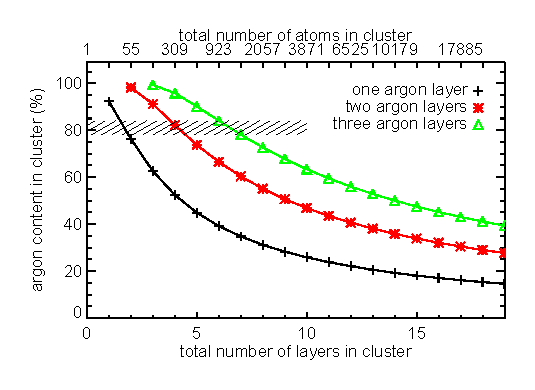
\includegraphics[width=8.2cm]{pics/figure_layers.pdf}
 \caption{
 Argon content of ideal icosahedric Xe-core, Ar-shell systems. 
 The relative number of surface atoms decreases with increasing cluster size.
 The hatched area corresponds to the Ar content of the largest clusters produced in our experiments (label `XL').
 \label{figure:layers}
 }
\end{figure}
%
For icosahedric clusters, the number of atoms in every shell is given.\cite{Mackay}
For a core-shell system in this ideal geometry, the relative content of both species can therefore readily be calculated.
In Figure \ref{figure:layers} we draw the Ar content of Xe-core, Ar-shell systems with one, two and three full Ar outer layers. 
A comparison of these graphs with Tables 1 and 3 of the main article shows that the largest clusters produced in our experiments (`XL'), for which a core-shell structure is probable, may have between 923 and 1415 atoms in total, corresponding to three and four Xe shells around a central Xe atom, followed by three Ar outer layers.
The Xe content for these systems is 0.16 and 0.22, resp.
%
%
\section{Electron-electron coincidence spectra}
%
%
In this work, we use electron-electron coincidence spectroscopy to isolate electrons from autoionization decays of Ar 3s$^{-1}$ vacancies from the remainder of the electron spectrum, mostly photoelectrons from outer valence levels and secondary electrons from intracluster inelastic collisions.
By recording two electrons ejected in the same process, on an event-by-event basis, we are able to identify those secondary electrons which are ejected after Ar 3s photoionization.
Here, we show a more detailed representation of the electron-electron coincidence data, from which figures in the main paper showing the ICD/ETMD spectra, and the pertaining Ar 3s photoelectron spectra, were derived.

A necessary condition for the ejection of two electrons by a single photon, irrespective of the mechanism by which this is accomplished, is a sufficiently high photon energy. 
In case of a sequential process, such as photoionization followed by ICD/ETMD, moreover the ionic state which is produced in the primary step must be located above the ionization threshold for the doubly ionized systems.
For Ar 3s autoionization, these conditions are discussed in detail in the main paper.
For a general double ionization process, the required energy can be estimated as the sum of the single ionization energies of the final state holes (main paper, Table 3) plus the geometry-dependent Coulomb repulsion (main paper, Figure 1).
Roughly, 27 eV are needed to produce an Ar 3p$^{-1}$ Xe 5p$_{3/2}^{-1}$ state, and about 2-4 eV less for $\rm (Xe\ 5p^{-1})_2$ states.
For photon energies exceeding this limit, the excess energy can be distributed to any, or both, of the released electrons.
For photoionization followed by autoionization the energy imparted to the first electron is determined by the binding energy of the primary vacancy, however.
This can be used to identify the pertaining second-step spectrum.

\begin{figure}
 \centering
 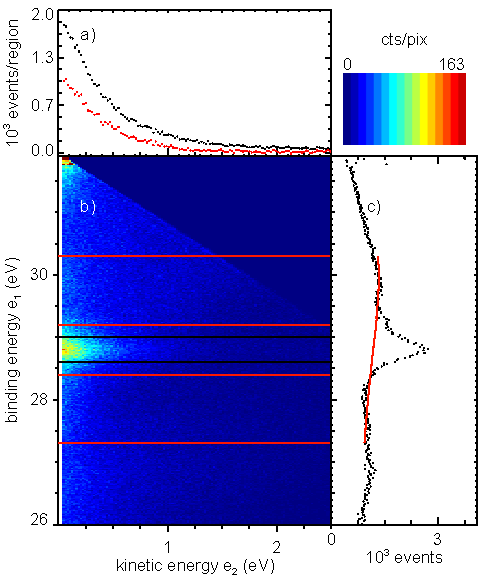
\includegraphics[width=12cm]{pics/figure_map.pdf}
 \caption{
Photon excited electron-electron coincidence spectrum of mixed Ar-Xe clusters (3\,\% Xe in the initial gas mixture) in the region of Ar inner valence electrons. 
(b): Color-coded map of coincident electron pairs, with the electron of higher kinetic named $e_1$. 
The energy of $e_1$ is given as binding energy, using the photon energy of $h\nu = 32$~eV. 
(c): Energy spectrum of primary electrons $e_1$, irrespective of the energy of the secondary electron (summation of the coincidence map along horizontal lines). 
(a): Energy spectrum of all secondary (ICD or ETMD) electrons $e_2$ pertaining to the Ar 3s binding energy region marked by two black bars. 
See text for details. 
Intensity is expressed as coincident events/pixel of 20~meV$^2$ (b) or as coincident events per interval of 20~meV (a,c). 
In total, approx. 4$\times 10^5$ events are shown. 
The color scale of (b) is linear.
 \label{figure:map}
 }
\end{figure}
%
Figure\ \ref{figure:map}b shows a typical electron-electron coincidence spectrum recorded with a photon energy of 32 eV, a few eV above the inner valence ionization thresholds.

The Figure shows that a significant amount of slow electrons $e_2$ are recorded in coincidence with the primary 3s electrons ($e_1$), which have a kinetic energy of approx. 3.3 eV. 
Some background of electron pairs at other energies is also visible.
It results from inelastic scattering of outer valence photoelectrons, and (in particular for the feature which has both electrons with kinetic energy less than 0.2 eV, upper left corner of Figure \ref{figure:map}b) due to inelastic scattering at parts of the analyzer.

More conventional, one-dimensional electron spectra pertaining to the photoelectrons and the ICD/ETMD electrons are obtained by summing up along one of the energy axis of the two-dimensional map, and are shown in (c) and (a). 
The peak in Figure \ref{figure:map}c at a binding energy of 28.7~eV pertains to the Ar 3s photoelectron line.
No atomic counterpart of this line is visible in this Figure, as only the cluster photoelectrons lead to electron-electron coincidences.
The trace shown in Figure \ref{figure:map}a is interpreted as the spectral shape of ICD/ETMD decays.

We have subtracted the background from random coincidences and coincidences due to inelastic electron scattering (electron impact ionization) from the signals shown in Figures \ref{figure:map}a,c.
In order to do so, the regions marked by the two pairs of red, horizontal bars in Figure \ref{figure:map}b were identified as background.
The coincidence map was then subdivided into intervals of 0.5 eV width in the $e_2$ energy coordinate.
For each interval, a second order polynomial was fitted to the background signal, and subsequently subtracted from the ICD/ETMD signal marked by the black, horizontal bars.
The summation of all background signals is shown as a wavy, solid red line in Figure \ref{figure:map}c, and the signal of secondary electrons, background subtracted, is shown as the lower trace of data points in Figure \ref{figure:map}a.
Background subtracted ICD/ETMD signals are shown throughout the main paper.

These data were recorded under all expansion conditions listed in Table 1.
A more detailed description of methods for analysing the data sets has been given.\cite{Foerstel_phd}
%
%
\section{Experimental ICD/ETMD spectra}
%
\begin{figure}
 \centering
 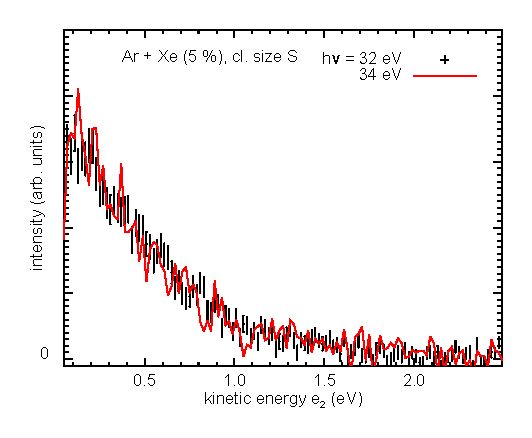
\includegraphics[width=13.12cm]{pics/630_631_cs.pdf}
 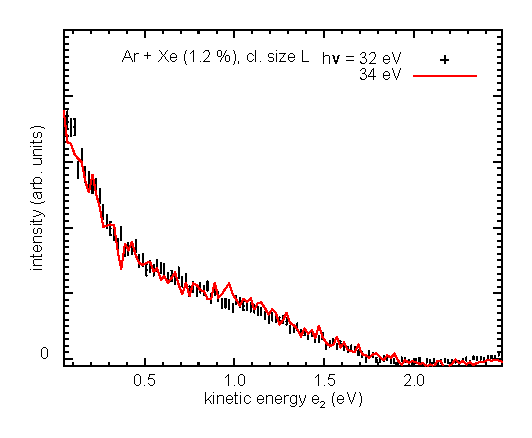
\includegraphics[width=13.12cm]{pics/673_674_cs.pdf}
 \caption{
Photon excited secondary electron spectra of mixed Ar-Xe clusters.
Spectra pertain to ICD and ETMD electrons with kinetic energy $e_2$ that are emitted after photoionization of an Ar 3s electron.
Excitation energies of $h\nu = 32$~eV (symbols) and $h\nu = 34$~eV (traces) are compared.
For comparison, spectra in each panel were normalized to equal area. 
(a) small clusters, 5\,\% Xe in the initial gas mixture.
(b) large clusters, 1.2\,\% Xe in the initial gas mixture.
 \label{figure:hnucomp}
 }
\end{figure}
%
The background subtracted signal of secondary electrons (of kinetic energy $e_2$) recorded in coincidence with a primary Ar 3s photoelectron (of kinetic energy $e_1$) is interpreted as the energy spectrum of ICD/ETMD of the cluster ensemble under study.
Some representative examples for such spectra are shown in the main article.
Here, we present a full account of these spectra.
For better comparison, similar to the article they have been arranged into groups of spectra from either clusters of equal size, or of equal composition of the gas mixture (resulting in a similar ratio of condensed Ar to Xe, at least when averaged over the cluster ensemble).
Thus, identical spectra appear more than once in the presentation.

As expected, the shape of the coincident $e_2$ spectra does not depend on the excitation energy (examples: Figure \ref{figure:hnucomp}).
For an excitation photon energy of $h\nu = 34$~eV, $e_2$ energies up to at least four eV can be observed in coincidence with an Ar 3s primary photoelectron.
No secondary electrons with energies exceeding two eV are observed however.

\begin{figure}
 \centering
 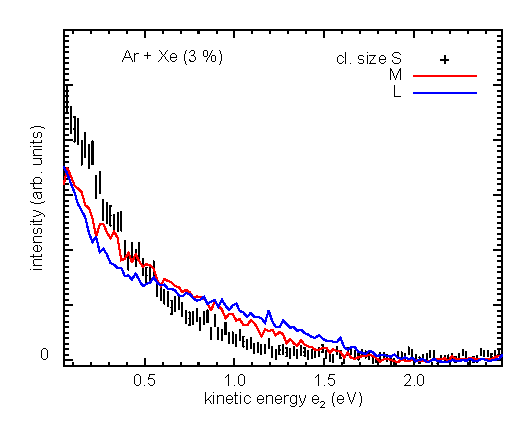
\includegraphics[width=8.2cm]{pics/661_653_cs.pdf}
 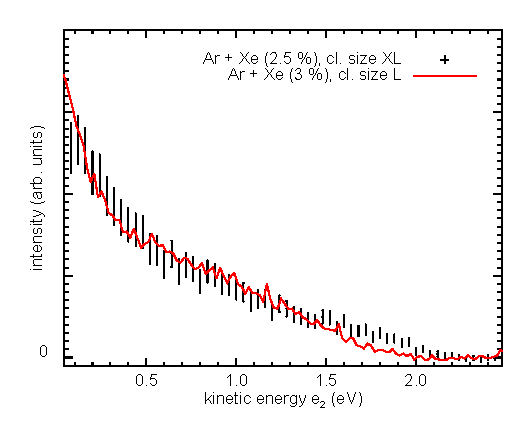
\includegraphics[width=8.2cm]{pics/867_658_cs.pdf}
 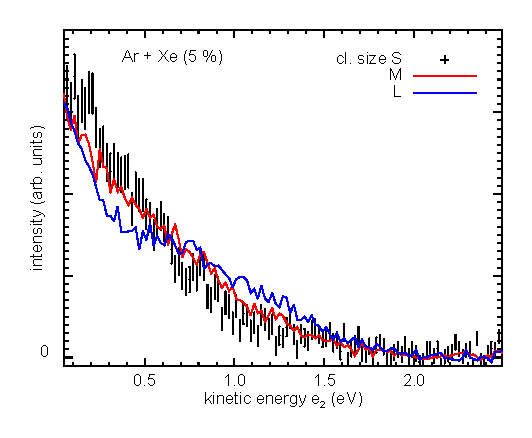
\includegraphics[width=8.2cm]{pics/630_998_cs.pdf}
 \caption{
Same as Figure \protect\ref{figure:hnucomp}.
Comparison of the spectra from cluster ensembles of different mean size.
Spectra were recorded at $h\nu = 32$~eV and were normalized to equal area. 
(a) small to large clusters, 3\,\% Xe in the initial gas mixture.
(b) very large and large clusters, 2.5\,\% Xe or 3\,\% Xe in the initial gas mixture, resp.
(c) small to large clusters, 5\,\% Xe in the initial gas mixture.
 \label{figure:sizcomp}
 }
\end{figure}
%
%
\begin{figure}
 \centering
 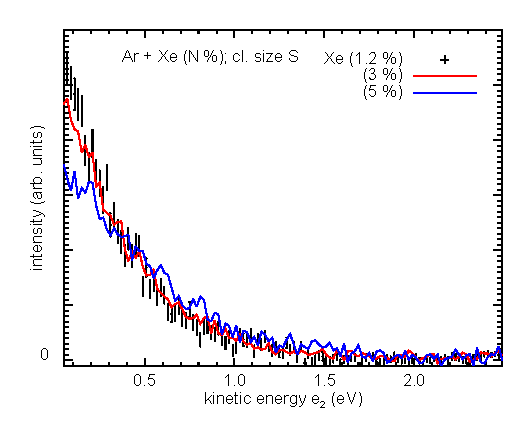
\includegraphics[width=8.2cm]{pics/677_661_cs.pdf}
 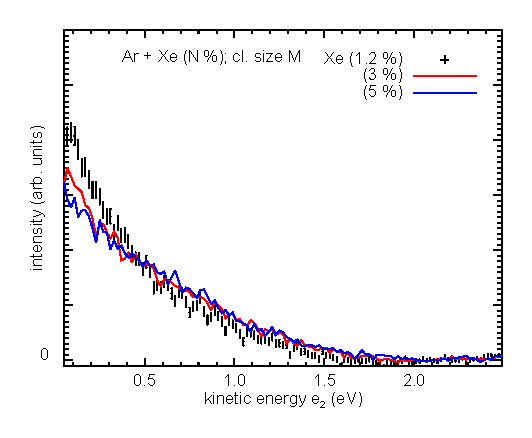
\includegraphics[width=8.2cm]{pics/668_653_cs.pdf}
 \caption{
Comparison of the spectra from cluster ensembles of different gas composition, see Figure \protect\ref{figure:sizcomp} for details.
(a) small cluster, 1.2-5\,\% Xe in the initial gas mixture.
(b) medium-sized clusters, 1.2-5\,\% Xe in the initial gas mixture.
 \label{figure:compcomp}
 }
\end{figure}
%
%
As discussed in the main paper, the differences between clusters of different size (Figure \ref{figure:sizcomp}) are more substantial than those between clusters of different gas composition (Figure \ref{figure:compcomp}).



\clearpage
\section{Additional Theoretical ICD/ETMD3 Spectra}

\subsection{Clusters with $N=38$ Atoms of Different Composition}
Recently, structures for ArXe clusters of in total 38 atoms were optimized
using an evolutionary algorithm based on two-body potentials determined
by xyz. \cite{marques}
In this section, the simulated ICD and ETMD3 spectra for selected cluster
structures shown in Figure 7 of Ref. \citenum{marques} are shown in Figures
\ref{figure:ArXe_lt15} -- \ref{figure:ArXe_gt50} and discussed.


\begin{figure}
 \centering
 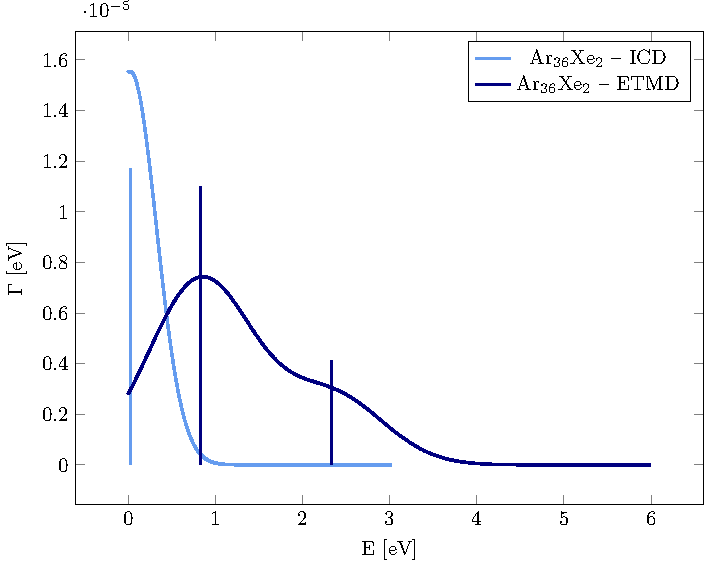
\includegraphics[width=0.32\columnwidth]{pics/Ar36Xe2.pdf}
 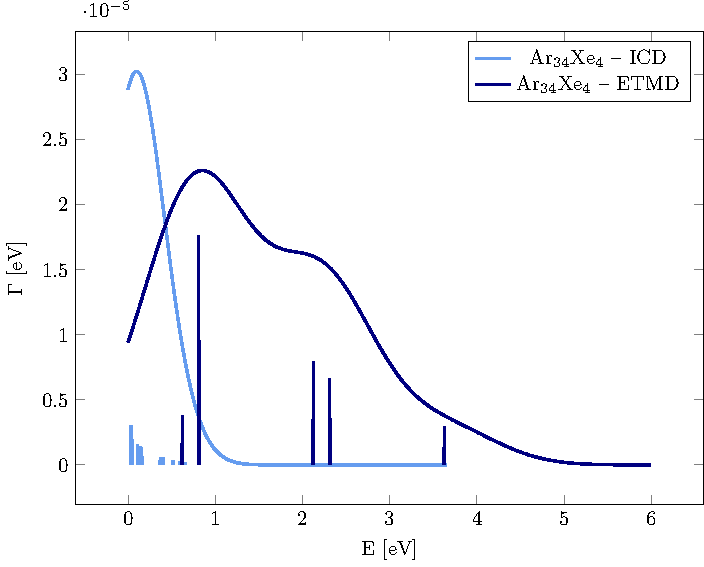
\includegraphics[width=0.32\columnwidth]{pics/Ar34Xe4.pdf}
 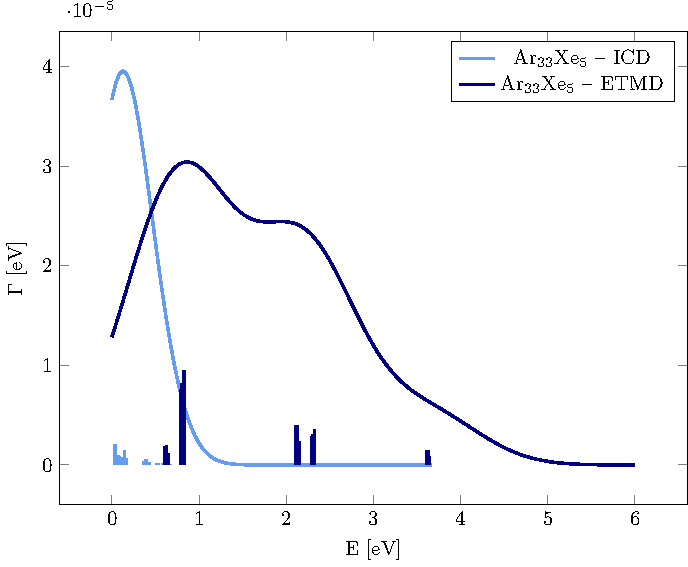
\includegraphics[width=0.32\columnwidth]{pics/Ar33Xe5.pdf}
 \caption{Ar$_N$Xe$_{38-N}$ clusters with a xenon content of
          \unit[5]{\%} to \unit[13]{\%}.
          According to our simulations the ETMD3 is the most prominent decay
          process for these cluster structures.
          In case of the Ar$_{36}$Xe$_2$ cluster only Xe-Xe distance is
          realized and therefore, the ETMD3 spectrum is very similar
          to one of a trimer
          showing two peaks originating
          from three different decay channels. In the other two cases the ETMD3
          spectrum is slightly more complex, but in all three cases, the ETMD3
          is manifested by peaks between \unit[0.5]{eV} and \unit[4.0]{eV} being
          in contrast to the experimental observations.}
 \label{figure:ArXe_lt15}
\end{figure}

\begin{figure}
 \centering
 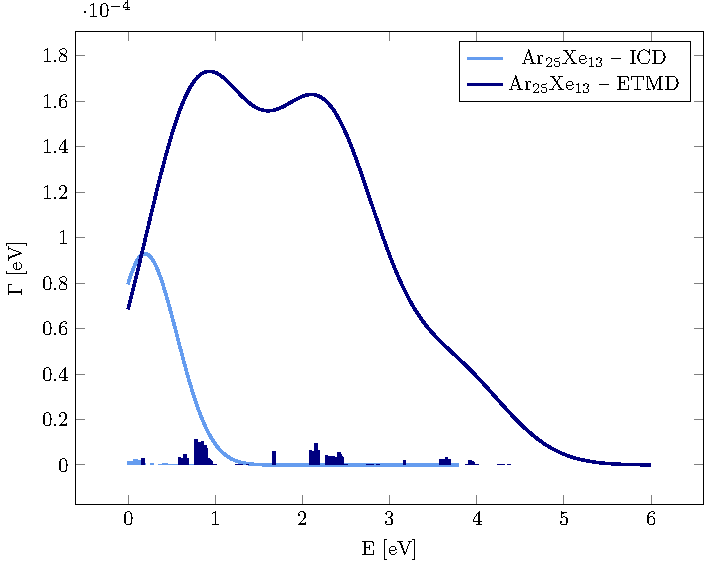
\includegraphics[width=0.5\columnwidth]{pics/Ar25Xe13.pdf}
 \caption{}
 \label{}
\end{figure}

\begin{figure}
 \centering
 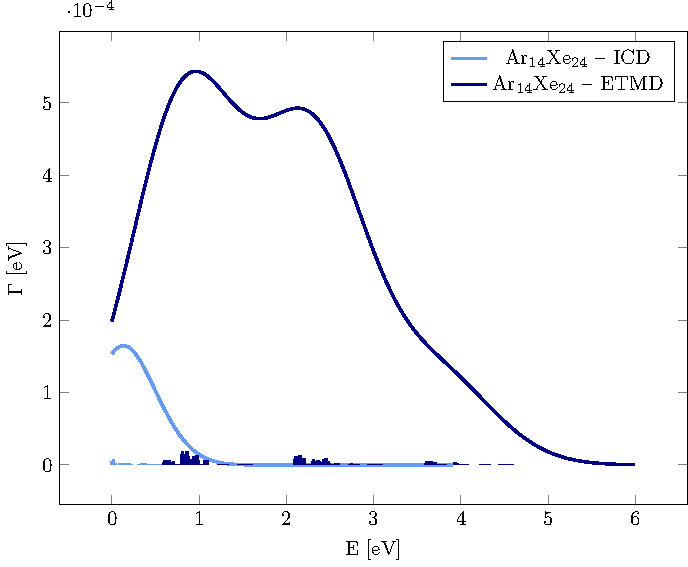
\includegraphics[width=0.5\columnwidth]{pics/Ar14Xe24.pdf}
 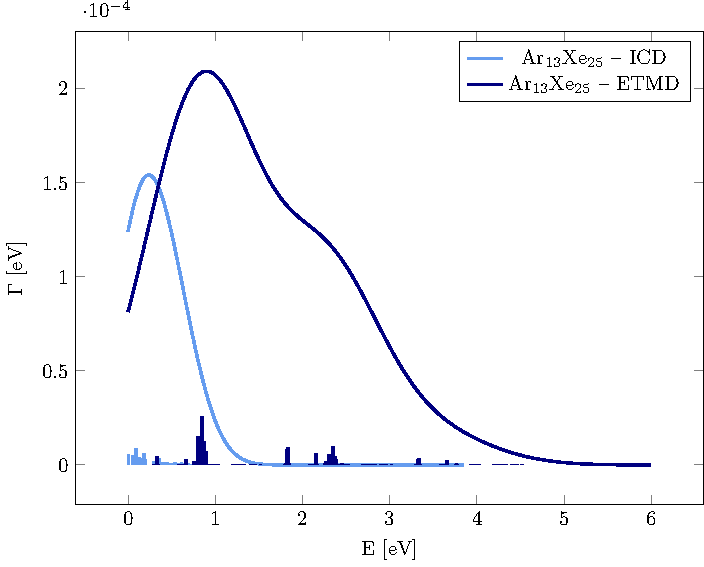
\includegraphics[width=0.5\columnwidth]{pics/Ar13Xe25.pdf}
 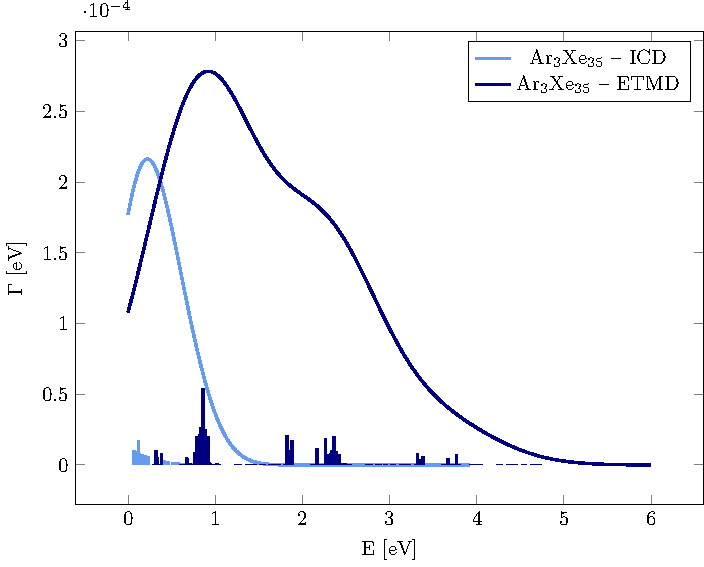
\includegraphics[width=0.5\columnwidth]{pics/Ar3Xe35.pdf}
 \caption{Ar$_N$Xe$_{38-N}$ clusters with a xenon content of more
          than \unit[50]{\%}.
          Our simulations show that ETMD3 is the dominant process
          for these cluster structures.
          They are shown for completeness but can, due to the high xenon content,
          not be related to the experimental secondary electron measurements.}
 \label{figure:ArXe_gt50}
\end{figure}


For all these cluster structures the ETMD3 is the more probable decay process and
except for the Ar$_{36}$Xe$_2$ case with \unit[43.6]{\%} ICD, the ETMD3 is clearly
the dominant process (compare Table xyz of the main article).
This can be explained by a combination of high xenon content and the
scattered distribution of the xenon atoms within the cluster structures.
Since the decay width of the ETMD3 is mostly caused by the decay
with direct neighbours and for these $\Gamma_{ETMD3} \propto N_{Ar} N_{Xe}^2$
both the maximization of direct xenon neighbours of an argon atom and the
maximization of the number of argon atoms being surrounded by xenon atoms
leads to a strong increase of the ETMD3 decay width. This situation is realized
in cluster structures without a seggregation of the two different elements like
in the structures of Ref. \cite{}. At the same time, all ICD channels are closed
for direct xenon neighbours. Therefore, a higher number of direct xenon neighbours
for all argon atoms reduces the number of possible decay partners for a given
cluster composition and therefore the ICD decay width.



%\begin{figure}
% \centering
% \includegraphics[width=0.5\columnwidth]{pics/ArXe.pdf}
% \caption{}
% \label{}
%\end{figure}
%
%\begin{figure}
% \centering
% \includegraphics[width=0.5\columnwidth]{pics/ArXe.pdf}
% \caption{}
% \label{}
%\end{figure}



%%%%%%%%%%%%%%%%%%%%%%%%%%%%%%%%%%%%%%%%%%%%%%%%%%%%%%%%%%%%%%%%%%%%%
%% The appropriate \bibliography command should be placed here.
%% Notice that the class file automatically sets \bibliographystyle
%% and also names the section correctly.
%%%%%%%%%%%%%%%%%%%%%%%%%%%%%%%%%%%%%%%%%%%%%%%%%%%%%%%%%%%%%%%%%%%%%
\raggedright
\bibliography{arxe}

\end{document}
